% do not change these two lines (this is a hard requirement
% there is one exception: you might replace oneside by twoside in case you deliver 
% the printed version in the accordant format
\documentclass[11pt,titlepage,oneside,openany]{article}
\usepackage{times}


\usepackage{graphicx}
\usepackage{latexsym}
\usepackage{amsmath}
\usepackage{amssymb}

\usepackage{ntheorem}

% \usepackage{paralist}
\usepackage{tabularx}

% this packaes are useful for nice algorithms
\usepackage{algorithm}
\usepackage{algorithmic}

% well, when your work is concerned with definitions, proposition and so on, we suggest this
% feel free to add Corrolary, Theorem or whatever you need
\newtheorem{definition}{Definition}
\newtheorem{proposition}{Proposition}


% its always useful to have some shortcuts (some are specific for algorithms
% if you do not like your formating you can change it here (instead of scanning through the whole text)
\renewcommand{\algorithmiccomment}[1]{\ensuremath{\rhd} \textit{#1}}
\def\MYCALL#1#2{{\small\textsc{#1}}(\textup{#2})}
\def\MYSET#1{\scshape{#1}}
\def\MYAND{\textbf{ and }}
\def\MYOR{\textbf{ or }}
\def\MYNOT{\textbf{ not }}
\def\MYTHROW{\textbf{ throw }}
\def\MYBREAK{\textbf{break }}
\def\MYEXCEPT#1{\scshape{#1}}
\def\MYTO{\textbf{ to }}
\def\MYNIL{\textsc{Nil}}
\def\MYUNKNOWN{ unknown }
% simple stuff (not all of this is used in this examples thesis
\def\INT{{\mathcal I}} % interpretation
\def\ONT{{\mathcal O}} % ontology
\def\SEM{{\mathcal S}} % alignment semantic
\def\ALI{{\mathcal A}} % alignment
\def\USE{{\mathcal U}} % set of unsatisfiable entities
\def\CON{{\mathcal C}} % conflict set
\def\DIA{\Delta} % diagnosis
% mups and mips
\def\MUP{{\mathcal M}} % ontology
\def\MIP{{\mathcal M}} % ontology
% distributed and local entities
\newcommand{\cc}[2]{\mathit{#1}\hspace{-1pt} \# \hspace{-1pt} \mathit{#2}}
\newcommand{\cx}[1]{\mathit{#1}}
% complex stuff
\def\MER#1#2#3#4{#1 \cup_{#3}^{#2} #4} % merged ontology
\def\MUPALL#1#2#3#4#5{\textit{MUPS}_{#1}\left(#2, #3, #4, #5\right)} % the set of all mups for some concept
\def\MIPALL#1#2{\textit{MIPS}_{#1}\left(#2\right)} % the set of all mips


% custom stuff
\usepackage{hyperref}


\begin{document}

\pagenumbering{roman}
% lets go for the title page, something like this should be okay
\begin{titlepage}
	\vspace*{2cm}
  \begin{center}
   {\huge Project Report \\}
   \vspace{2cm} 
   {\Large Student Project Semantic Web Technologies HWS18\\}
   \vspace{2cm}
   {\Large Presented by \\}
   \vspace{0.5cm}
    {
    Nele Ecker\\
    Alex L\"utke\\
    Marvin Messenzehl \\
   }
   \vspace{1cm} 
   { Submitted to the\\
    Data and Web Science Group\\
    Prof.\ Dr.\ Heiko Paulheim \& Sven Hertling \\
    University of Mannheim\\} \vspace{2cm}
   {October - December 2018}
  \end{center}
\end{titlepage} 

% no lets make some add some table of contents
\tableofcontents
\newpage

%\listofalgorithms

%\listoffigures

%\listoftables

% evntuelly you might add something like this
% \listtheorems{definition}
% \listtheorems{proposition}

%\newpage


% okay, start new numbering ... here is where it really starts
\pagenumbering{arabic}

%%%%%%%%%%%%%%%%%%%%%%%%%%%%%%%%%%%%%%%%

% INPUTS
\section{Application Domain and Goals}

\subsection{Problem Statement And User Needs}
Everyone who does regular city trips knows the problem. You visit a foreign city and just don’t get the same experience as people who live there and know the place well. Typical information sources, like tourist centers, provide a very biased opinion on what one should see and what not. But what if somebody wants to look for something special or has special interests? If somebody really wants to get to know a city and the different districts,  this takes a lot of time and manual preparation. \\ \\
This problem should be solved within this project through an application that uses semantic web technologies. This application will be named \textit{Semaps - A semantic approach to maps.} 

\subsection{Application Goal}
The overall goal of the developed application is to give the user a visual help to easily identify the particularities of the different city districts. This should be done with the help of a map as the main user interface where the different districts are marked in different colors in the form of rectangles.
\\
Examples of this would be categories like \textit{shopping, tourists, universities} and a lot more. The detailed categories depend on the districts, building and the offer of the respective city. 
\\ \\
In the end, the user should visit the web application where he/she sees a map of a city where different special districts are marked. Therefore trips can be planned more individual and efficient.

\section{Datasets}
The application is based on two different datasets, namely LinkedGeoData and Dbpedia. It was decided to work with both datasets separately, due to the fact that LinkedGeoData is already very detailed and most data of Dbpedia is already in the other dataset. Having to different datasets allows the user to compare the results and can also give hints how accurate Dbpedia actually is. 

To get the data from LinkedGeoData, different approaches where tried. The first approach was to download all the data and use it offline. This soon appeared to be not sophisticating, because of multiple reasons. On the first hand the dataset is split, based on the main categories Amenity, SportThings, HistoricalThings, etc, with each subdataset having a large size and in case that you want to use all the data more than 40 datasets have to be loaded. On the other hand loading single datasets into a model when starting the application takes very long. Small datasets, for example all MilitaryThings need only a few seconds to be loaded, but others as for example HistoricThings need approximately one hour. As this is not feasible, to load every time that a user starts a request, it was decided to look for other ways to load the data. The most easiest way was to directly use the sparql endpoint of LinkedGeoData, which can be simply used in Jena. The used query can be found in \ref{fig:sparqlLGD}. 

\begin{figure}
	\centering
	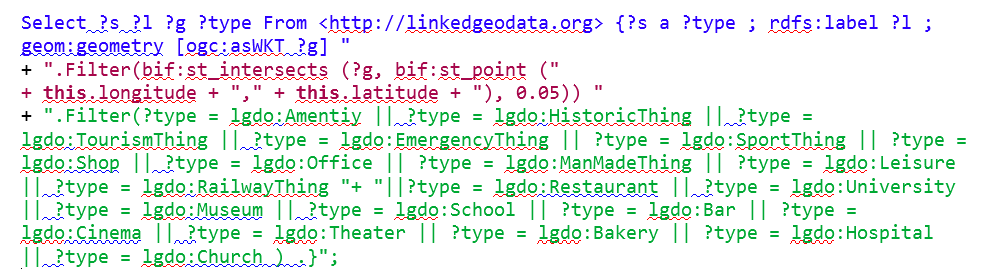
\includegraphics[scale=0.7]{./content/sparqlLGD.png}
	\caption{Sparql query to select all data of LinkedGeoData}\label{fig:sparqlLGD}
\end{figure}

The query consists of three parts which are differently colored. The blue part selects the values of the needed variables, while the red and the green part show two different filters. The first filter is used to not read the data of the whole world, but only in a given region. The region that should be used is defined by the user and then used by this.latitude and this.longitude. Using st\_intersects makes it possible to get all points that are in a specified radius around a given point. It was decided to use a 50km radius around the point that the user chose. 

In the first version of the application only the location filter was used. That allowed us to use all existing categories, what would have made the clustering very dynamic. But as there are many different categories, also some very general and thus for our use case uninteresting ones, the time to get all triples was too long. The requests were interrupted after 15 minutes waiting time, but in our opinion even a minute waiting time is not acceptable for the application. 

Due to these experiences the second filter was introduced, this time filtering the categories. Because of the separation of the dataset based on the main categories, as it is done for the download, we are already aware of the main categories which are also represented in the filter. Furthermore some more specialized categories, like museum and university are added, as they are more interesting for the clustering. Having the second filter the request needs only a few seconds, what makes the application usable.

To get the data of Dbpedia, the corresponding sparql endpoint was directly used. The query is shown in \ref{fig:sparqlDbpedia}. It is similar to the one used for LinkedGeoData, except a third filter was added, due to the fact that Dbpedia allows to have multiple labels for each resource with different language tags. Without using the language filter, there would be multiple instances for each class, one per label. Using the filter makes it sure that only the english label is used for the application and thus only one instance is created, as expected. Having multiple labels was not experienced using LinkedGeoData, that’s why the filter is not in the first query. Basically the same information was selected, except the longitude and latitude are read separately, as this worked better with the location filter. The filter on the categories has been modified, to filter the categories that are attached to a Dbpedia resource. The general idea of the types has not changed, as it is also possible to look for museums and universities, but the URIs are different. 

\begin{figure}
	\centering
	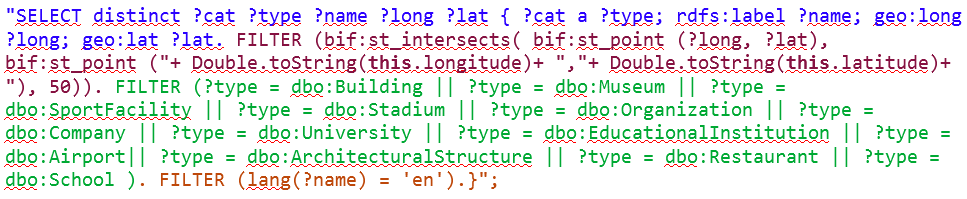
\includegraphics[scale=0.7]{./content/sparqlDbpedia.png}
	\caption{Sparql query to select all data of Dbpedia}\label{fig:sparqlDbpedia}
\end{figure}

While exploring the different resources of Dbpedia manually, one major issue for the application was found. Not all points of interest that can be found in Dbpedia have information about their location. These points can therefore not be used for the clustering and falsify the result comapared to LinkedGeoData.
\section{Techniques}
One of the main ideas during development was the decoupling of major steps in Semap’s processing pipeline. So the project is split into three smaller part: The user interface, the processing pipeline and REST interfaces. 
The frontend website is primarily responsible for the rendering of visual elements. The computation of clusters takes place on a separate backend server, which is contacted by the website using a REST-interface on the same backend server. The following sections will be based on this trisection and elaborate in more detail on each of the components.

\subsection{User Interface}


\subsection{REST Interface}
When a request is sent to the REST interface, the server reads given parameters and schedules the crawling and clustering of the data as well as the assembly of a response in the GeoJSON format. So the interface does not execute any functional computations; it rather passes on the request to different execution modules. The REST interface relies on the JAX-RS implementation, also known as Jersey with Java Servlet Annotations 3.0. On a server startup, a glassfish servlet container is created inside any webserver and requests to the webserver forwarded to the container. The container itself requires little configuration, as most of it is done by coding and Java 3.0 annotations. In the container, a usual servlet-container runs, which passes the requests to other components as described in the following sections. 

\subsection{Processing Pipeline}
A core object structure underlies the processing pipeline, which is utilized whenever the backend server is contacted by the UI website. I.e. After crawling the data from respective servers, the results are saved in internal object representations and read when the processing takes place. The core object structure is tuned towards the task of semantically clustering regions and thus facilitates the use of multiple clustering implementations with diverse libraries. The UML class diagram in figure \ref{fig:cos} summarizes the object structure:
 
\begin{figure}
  \centering
    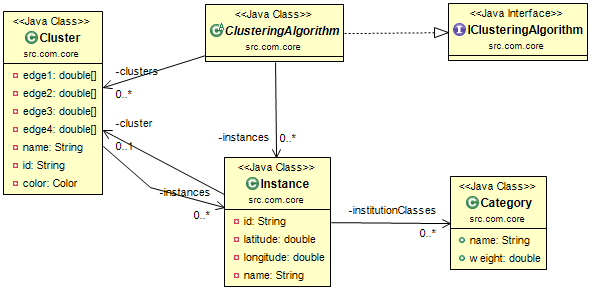
\includegraphics[scale=0.8]{./content/cos.png}
  \caption{UML class diagram of the core object structure}\label{fig:cos}
\end{figure}


The figure shows the centrality of the Instance class. All other attributes interact with it, as they rely on the information held in instance objects. Practically speaking, an instance represents a real-world institution like a specific bar or school. Each object of the instance class can have a number of Categories assigned to it. Categories make up the semantic context of an institution. They have a name like “museum” or “bar” and a weight. The semap project assumes, that the deeper a category is in its ontology, the more informative it is. That is why a detailed category like “Irish pub” is meant to get a higher weight than higher-level categories like “thing”. The clustering algorithm can then prefer to place instances based on the deep-level knowledge into clusters, resulting in more specific clusters.
Before clustering takes place, no instance is assigned to a cluster, as no cluster exists. Ideally after clustering each instance is assigned to exactly one cluster. When running a clustering algorithm (here represented by an abstract class), it will create new objects of type Cluster using a list of instances and assign those instances to a cluster. The different implementations of clustering algorithms are not depicted in the figure for abstraction purposes. But in the end, the actual implementations are of type ClusteringAlgorithm, so they just inherit from the abstract class ClusteringAlgorithm and the interface IClusteringAlgorithm. In the project, a simple square clustering algorithm and a DBScan were implemented.


\paragraph{Simple Square Clustering }
The simple square clustering algorithm a rather straight-forward implementation of clustering algorithms. It considers each element from the list of instances and creates clusters based on their position. So for each instance, the simple square clustering implementation will check if there is already a cluster, in which the current instance is located and will assign it to this cluster or create a new cluster correspondingly. After having done so for the entire list of instances, each clusters gets a category. The computation is based on a scoring function, which determines the times, a category appears in a cluster and weights each appearance by the category’s weight-property. The category with the highest weight is then allocated to a cluster. Algorithm \ref{alg:ssca} formalizes the procedures again. In sum, the simple square clustering algorithm does not take into account the semantic context (i.e. the categories) of instances and only uses positional information initially. That is why the results are not guaranteed to be semantically meaningful. However, the algorithm runs very fast, as it is linked to very little computational overhead.


\begin{algorithm}
\caption{Sketch of the simple quare clustering algorithm}\label{alg:ssca}
\begin{algorithmic} 
\STATE $I \gets \text{set~of~all~instances}$
\STATE $C \gets \emptyset$
\FORALL{$i \in I$}
\FORALL{$c \in C$}
 \IF{$i~located~in~c$}
  \STATE $c.add(i)$
  \ELSE 
  \STATE $x \gets createCluster(i.latitude, i.longitude)$
  \STATE $C \gets C \cap x$
\ENDIF
\ENDFOR
\ENDFOR
\STATE ${CAT} \gets \emptyset$
\FORALL{$c \in C$}
\FORALL{$i \in C.getInstances()$}
\FORALL{$category \in i.getCategories()$}
\STATE ${CAT}_{category} \gets {CAT}_{category}.getScore() + category.getScore()$
\STATE ${CAT} \gets {CAT} \cap {CAT}_{category}$
\ENDFOR
\ENDFOR
\ENDFOR
\RETURN $max({CAT}.getAllScores())$
\end{algorithmic}
\end{algorithm}

\paragraph{DBScan}
DBScan is a the sophisticated clustering algorithm in the semap project and relies on the Weka library implementation. The DBScan tries to build clusters based on two pieces of information: The position of instances and their categories. The position is determined by the longitude and latitude coordinates and is normalized on a scale from zero to one; alternatively it can be z-normalized by a parameter setting in the Java coding. Categories are one-hot-encoded, so that each instance gets a vectors consisting of values in the range from one to zero. The vector represents the set of all categories. Each category is represented by a positional value in the vector. All the categories an instance does not belong to, take the value 0 in the vector. The categories, an instance belongs to, take a normalized value greater than zero. The value is determined by the formula: 
\begin{equation}
n := number~of~categories~of~an~instance
\end{equation}
\begin{equation}
w_i := weight~of~the~i\-th~category~of~an~instance
\end{equation}
\begin{equation}
w_c := weight~of~current~category
\end{equation}
\begin{equation}\label{eq:normalization}
val = \frac{w_c}{\sum_{i=0}^{n}w_i}
\end{equation}


Weight of current category/sum of categories of an instance(weight)
So the value depends on the number of instance’s categories and the weight of the respective categories. This method ensures, that the weighted vector values have the same impact on the clustering as the positional information latitude and longitude. Before the DBScan algorithm can start working in Weka, a preprocessing pipeline transform the internal object representation as described in figure \ref{fig:cos} into the object representation needed by the Weka library. It therefore writes an artificial .arff-file to disk and reads it again with tools from the weka library. Afterwards, the DBScan is executed and the results again returned into the core object representation of semap. The entire procedure of the DBScan in the semap project is summarized in algorithm \ref{alg:dbscan} as follows:

\begin{algorithm}
\caption{Sketch of the DBScan clustering algorithm}\label{alg:dbscan}
\begin{algorithmic} 
\STATE $I \gets \text{set~of~all~instances}$
\STATE $C \gets \emptyset$
\FORALL{$i \in I$}
\STATE $x \gets normalize(i.latitude)$
\STATE $i.setLatitude(x)$
\STATE $x \gets normalize(i.longitude)$
\STATE $i.setLongitude(x)$
\STATE $\vec{y} \gets oneHotEncode(i.categories)$
\FORALL{$z \in \vec{y}$}
\STATE $z \gets normalize~z~as~to~formula~(\ref{eq:normalization})$
\ENDFOR
\STATE $i.setLatitude(x)$
\ENDFOR
\STATE ${CAT} \gets \emptyset$
\FORALL{$c \in C$}
\FORALL{$i \in C.getInstances()$}
\FORALL{$category \in i.getCategories()$}
\STATE ${CAT}_{category} \gets {CAT}_{category}.getScore() + category.getScore()$
\STATE ${CAT} \gets {CAT} \cap {CAT}_{category}$
\ENDFOR
\ENDFOR
\ENDFOR
\RETURN $max({CAT}.getAllScores())$
\end{algorithmic}
\end{algorithm}

In sum, the value normalization and object transformations are computationally expensive operations. While for example the simple square algorithm clusters multiple millions of instances within few milliseconds, the DBScan requires about 30 seconds to do so with only 15 thousand instances. However, the major part of this timeframe is not spent in the normalization and object transformation implementation. The most time is actually needed by Weka’s DBScan algorithm itself. So this runtime behavior is a major limitation of the DBScan algorithm. Nonetheless, the DBScan algorithm is capable of finding much more meaningful results. It considers categories of instances already when performing the clustering and not afterwards. It is also not limited to geographically speaking squared clusters, but has arbitrary decision boundaries. That makes this algorithm a very powerful tool for detailed analyses on regional, public data.


\section{Results}
What outcomes does the application provide? \\
How are some user queries answered?

Evaluation, based on Mannheim sample:
\begin{figure}
  \centering
    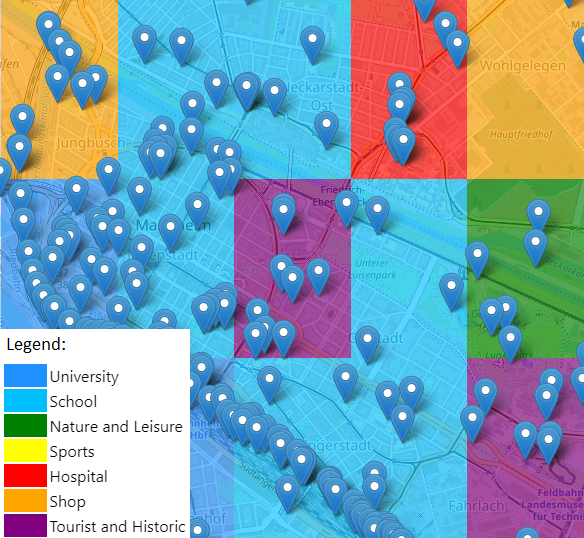
\includegraphics[scale=0.75]{./content/sample.PNG}
  \caption{Evaluation based on sample result in Mannheim}\label{fig:eval}
\end{figure}

\section{Known Limitations}
In which domains does the application not work? \\
Are there queries which cannot be answered? \\
Why? \\
How could you overcome those limitations, given more time?
\section{Lessons Learned}
Which challenges did you face? \\
What were the biggest obstacles? \\
What would you do different the next time?



\newpage


\pagestyle{empty}


%\section*{Ehrenw\"ortliche Erkl\"arung}
%Ich versichere, dass ich die beiliegende Master-/Bachelorarbeit ohne Hilfe Dritter
%und ohne Benutzung anderer als der angegebenen Quellen und Hilfsmittel
%angefertigt und die den benutzten Quellen w\"ortlich oder inhaltlich
%entnommenen Stellen als solche kenntlich gemacht habe. Diese Arbeit
%hat in gleicher oder \"ahnlicher Form noch keiner Pr\"ufungsbeh\"orde
%vorgelegen. Ich bin mir bewusst, dass eine falsche Er- kl\"arung rechtliche Folgen haben
%wird.
%\\
%\\

%\noindent
%Mannheim, den 31.08.2014 \hspace{4cm} Unterschrift

\end{document}
